\section{Search for non-lithium electrolytes}

Nowadays, the demand for power storage systems is increasing, mainly due to the growth of the mobile devices and the electric cars market~\cite{energy-demand}. One of the most popular types of energy source in everyday use are lithium-ion batteries (LIBs), widely used in portable electronics, such as notebooks, smartphones, etc.~\cite{energy-storage}. This is due to the relatively high standard potential of the Li/Li$^{+}$ pair and the low lithium density. Early research showed that the presence of metallic lithium in the battery can cause explosions, so the standard LIB used graphite as the anode and cobaltium oxide as the cathode~\cite{lib-review}. In recent years, some improved electrode materials for LIBs were developed~\cite{lib-review-2}. As an electrolyte in such batteries, LiPF$_6$ solution in a~mixture of ethylene carbonate (EC) and dimethyl carbonate (DMC) or lithium salts solutions in ionic liquids are commonly used~\cite{lib-electrolytes}. Systems based on poly(ethylene oxide) (PEO) were also studied, due to their safety, ease of fabrication, and low cost~\cite{lib-peo-electrolytes}.

\begin{table}
    \centering
    \caption{Abundance of example elements in the earth crust~\cite{lithium-abundance}}
    \begin{tabular}{ccc}
        \toprule
         &  \multicolumn{2}{c}{Abundance in earth crust [ppm]} \\
        Element & Upper & Lower \\
        \midrule
        Na & 25670 & 21200 \\
        Mg & 13510 & 31550 \\
        V & 53 & 149 \\
        Zn & 52 & 79 \\
        La & 32.3 & 26.8 \\
        Nd & 25.9 & 28.1 \\
        Li & 22 & 13 \\
        Nb & 26 & 11.3 \\
        Ga & 14 & 17 \\
        \bottomrule
    \end{tabular}    
    \label{tab:lithium_abundance}
\end{table}

Despite the efficiency of LIBs in energy storage, there exists a~possible danger to their widespread use, due to the limited abundance of lithium in earth crust~\cite{lithium-abundance}. The abundance of sample elements is presented in Table~\ref{tab:lithium_abundance}. What can be observed is the fact that lithium is not so widespread and its content in earth crust is of the same order of magnitude as for elements usually considered as rare, like neodymium or gadolinium. Furthermore, its deposits are mainly located in countries in Africa and South America as well as China and Russia, which may cause political problems with stability of deliveries~\cite{lithium-shortage}. However, there are also opinions that lithium shortage is not a~serious threat~\cite{lithium-contra}.

The problems mentioned with lithium supplies are one of the reasons why since early 2010s a~large effort is put into research of alternative batteries using elements which are quite common and widespread, such as sodium~\cite{na-ion-1,na-ion-2,na-ion-3,na-ion-4,na-ion-5} or magnesium~\cite{mg-ion-1,mg-ion-2,mg-ion-3,mg-ion-4,mg-ion-5,mg-ion-6,mg-ion-7,mg-ion-8,mg-ion-9}. An additional advantage of this approach is that sodium-based systems are friendly to the environment~\cite{na-environment}.

Due to similar chemical properties of sodium and lithium, materials used in LIBs were also studied for sodium-ion batteries, nevertheless, there were some differences in properties because of larger size and different bonding characteristics of sodium compared to lithium~\cite{li-na-comparison}. In sodium-based batteries technology, pyrolized carbon compounds, derivatives of titanium oxide~\cite{na-ion-1}, transition metal sulfides~\cite{na-ion-5}, tin-antimonium alloys~\cite{na-ion-2} were considered as anodes and doped oxides of cobalt, vanadium or manganese, transition metal phosphates, fluorides~\cite{na-ion-1}, sulfides~\cite{na-ion-2} and hexacyanoferrates~\cite{na-ion-5} were proposed as catode materials. For magnesium-based batteries, pure magnesium~\cite{mg-ion-1} (although with complications related to the formation of the passivation layer~\cite{mg-ion-10}), alloys of bismuth and antimony~\cite{mg-ion-11} or tin~\cite{mg-ion-12} were considered as anodes, while catodes were mostly based on transition metal oxides such as cobalt~\cite{mg-ion-14}, vanadium~\cite{mg-ion-15}, manganese~\cite{mg-ion-17}, ruthenium~\cite{mg-ion-13} or molybdenium~\cite{mg-ion-16}. Unlike LiPF$_6$ dissolved in a~mixture of EC and DMC, which is a~standard electrolyte for LIBs, the case of an optimal electrolyte for non-lithium batteries is still a~subject of research. Such system, to be applicable for use in batteries, should fulfill some requirements~\cite{na-ion-4}:
\begin{itemize}
    \item chemical stability --- no side chemical reactions during cell utilization,
    \item electrochemical stability --- its components should have HOMO-LUMO gap large enough to not undergo redox processes during cell utilization,
    \item thermal stability --- it should be liquid or gel and do not decompose in the working temperature range,
    \item insensitive to contamination of water,
    \item be a~good ionic conductor and electronic insulator,
    \item non-toxic, cheap in production, environment-friendly.
\end{itemize}

The electrochemical stability condition limits the choice of the anion for the salt dissolved in the electrolyte, among them are anions that are also commonly used in lithium cells, such as BF$_4^{-}$, ClO$_4^{-}$, [N(FSO$_2$)$_2$]$^{-}$ (FSI) or [N(CF$_3$SO$_2$)$_2$]$^{-}$ (TFSI)~\cite{na-ion-4}. The last two are very valuable because NaFSI and NaTFSI are nontoxic, thermally stable, and their solutions have reasonable values of conductivity~\cite{na-fsi,na-il-1}. For magnesium-based electrolytes, very popular is the use of MgCl$_2$~\cite{mg-ion-7} (due to its low cost) or magnesium aluminium chloride complexes~\cite{mg-ion-6}.

Protic solvents are excluded because of the condition of electrochemical stability. One class of compounds studied are organic solvents and their mixtures with compositions aiming at improving stability and lowering viscosity. Among them are cyclic (EC) or linear (DMC) carbonates~\cite{el-carbonates}, nitriles~\cite{el-nitriles}, esters and ethers such as glymes~\cite{el-ethers-1,el-ethers-2,mg-ion-20}, imidazolium derivatives~\cite{el-imidazolium} and polymer systems based on poly(ethylene oxide) (PEO)~\cite{el-peo-1,el-peo-2,mg-ion-19}. Furthermore, fluorinated derivatives of solvents, e.g., EC fluorinated derivatives, were investigated due to their ability to lower the flammability of the electrolyte and improve its electrochemical stability~\cite{fluorination-1,fluorination-2,fluorination-3,fluorination-4}. From these solvents, one of the best mixtures was EC with propylene carbonate (PC) and either DMC or dimethoxyethane (DME)~\cite{na-ion-6,mg-ion-18}. It was also shown that the change in electrolyte properties can be made by using a~salt mixture, such as MgCl$_2$ and AlCl$_3$~\cite{mg-ion-6}. Another example are Mg(TFSI)$_2$ solutions in DME, where an addition of chloride anions in the form of MgCl$_2$~\cite{mg-cl-tfsi} improved its performance.

Another class of solvents considered are ionic liquids (ILs). In general, they are organic salts which are molten at ambient temperature. They are chemically and electrochemically stable~\cite{il-3}, have a~wide range of liquid state and very low vapor pressure, making them safe due to their nonflammability~\cite{il-stability}. ILs are composed entirely of ions; therefore, electrostatic interactions dominate their properties. In ILs, a wide choice of anions can be used, the systems most frequently studied are based on FSI$^{-}$ and TFSI$^{-}$ or simpler anions such as chlorides, bromides, iodides, nitrates, acetates, phosphates, tetrafluoroborates and hexafluorophosphates~\cite{il-1}. The proper choice of IL cation could improve the performance of the electrolyte; the most popular in recent studies are cations based on imidazolium (like 1-ethyl-3-methylimidazolium, briefly EMIM) or pyrrolidinium~\cite{na-il-1,na-il-2,na-il-3,na-il-4,na-il-5,na-il-6,na-il-7,na-il-8,na-il-9,na-il-10,na-il-11,mg-ion-13,mg-ion-14}. The usage of ILs is not limited to electrolytes, as they were also used as CO$_2$ absorbents~\cite{il-2}, catalysts in organic and inorganic synthesis, solvents for enzymes or lubricants~\cite{il-5}. A~common experimental problem with ILs is that they are usually contaminated with water~\cite{il-4}.

Research on "beyond lithium" chemistries is quite intense and several potentially interesting systems were found - some of the developed sodium-based electrolytes are better in terms of conductivity than lithium-based analogs~\cite{na-fsi}. Another alternative studied (although not as intensively as sodium or magnesium electrolytes) were systems based on zinc~\cite{na-il-10, zn-1, zn-2} or aluminum~\cite{al-1,al-2,al-3}.

Experimental research on electrolyte properties is conducted both at the local level - solvation shells and electrode/electrolyte interfaces - and at the macroscopic level, including density, viscosity, and ionic conductivity. Impedance spectroscopy with NMR spectroscopy are used for studying ion transport. For testing electrochemical stability, cyclic volammetry is usually applied. Safety features, such as temperature stability, vapor pressures or ignition temperatures, are studied with thermogravimetric analysis, differential scanning calorimetry, or accelerating rate calorimetry~\cite{na-ion-4}. Other examples of such research include structure determination by rentgenographic methods~\cite{roentgen-exp}, neutron diffraction~\cite{neutron-diffraction} or spectroscopy~\cite{spectroscopy-structure-1,spectroscopy-structure-2}. An example of such Raman spectrum is shown in Figure~\ref{fig:introduction-li-tfsi-raman}.

\begin{figure}[ht]
    \centering
    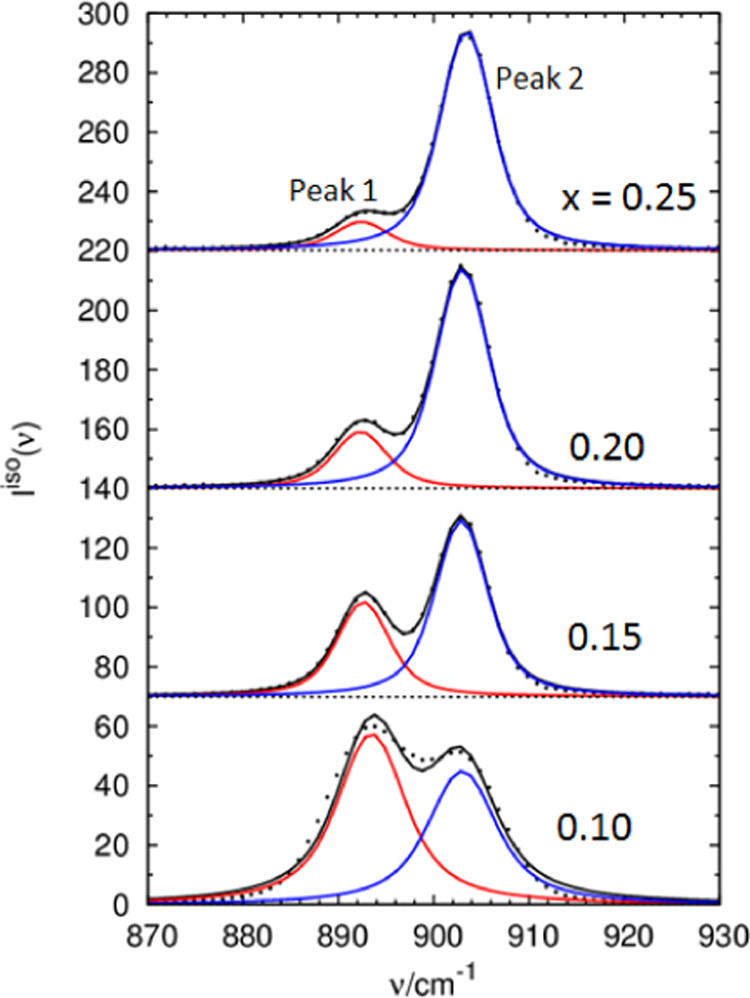
\includegraphics[width=0.55\textwidth]{img/1-introduction/li-tfsi-raman.png}
    \caption{Raman spectra of (LiTFSI)$_x$EC$_{1 - x}$ with different molar fraction $x$ of lithium salt, with deconvoluted bands for free and coordinated EC~\cite{neutron-diffraction}}
    \label{fig:introduction-li-tfsi-raman}
\end{figure}